\section{Related Works}


\begin{frame}{Efficient Toxic Content Detection by Bootstrapping and Distilling Large Language Models}

\begin{itemize}

  \item Several deep learning techniques have been developed to automate toxic content detection 

  \item \textbf{Supervised learning}: Predict a manually provided target output
    \begin{itemize}
      \item Performance of the system grows with the size of labelled data 
      \item Data and annotations are rare, costly, or time-consuming to collect
      \item Overfit to the training task
      \item  Lack the properties for knowledge transfer and generalization
    \end{itemize}

  \item \textbf{Large Language Models}: superior zero-shot and few-shot context learning performance and transferability.
  \begin{itemize}
    \item Designing novel prompting approaches to enhance the performance
  \end{itemize}

\end{itemize}

\end{frame}


\begin{frame}{Efficient Toxic Content Detection by Bootstrapping and Distilling Large Language Models}

  \begin{itemize}

  \item Performance relies heavily on the quality of prompts
  \item Deploying LLMs for toxic content detection can incur both high run-time costs and high latency 
  \item \textbf{Existing works}-Bootstrapping and Distilling LLM's
  \begin{itemize}
    \item Decision-Tree-of-Thought
    \item Fine-tune a suitable student LM with a smaller model size
  \end{itemize}
  \begin{figure}
    \centering
    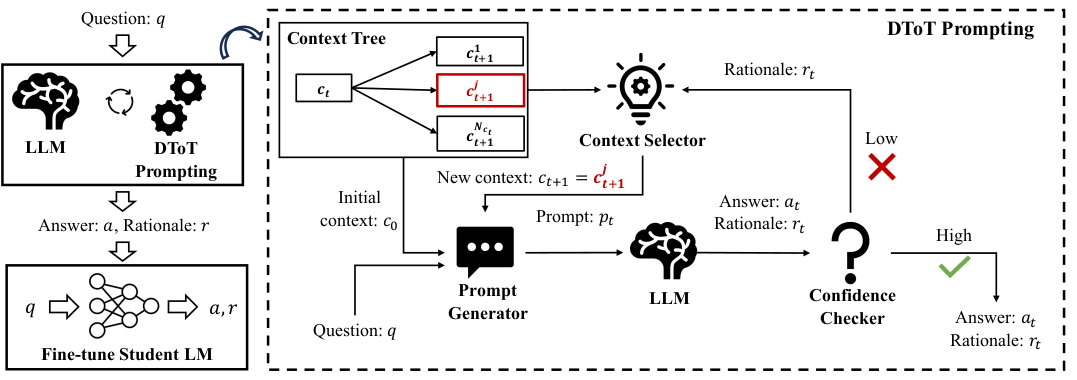
\includegraphics[width=1\linewidth]{images/BD_LLM.png}
    \caption{Illustration of BD-LLM}
    \label{fig:1}
  \end{figure}

\end{itemize}
    
\end{frame}


\begin{frame}{Toxicity Detection with Generative Prompt-based Inference}

\begin{itemize}
  \item Yau et al. use a generation-based approach to classify a text $x = (x_1, x_2, \dots, x_T)$.
  \item They claim that certain prompts steer the model towards generating toxic content, which they use to do so.
  \item Given such positive and negative prompts $y^p$ and $y^n$, they calculate the likelihood that $x$ is generated given $y \in \{y^p, y^n\}$ as:

  \[ s(y) = \sum_{t = 1}^{T} log ~ P_M(x_t | y, x_{<t}) \]

  \item If $s(y^p) > s(y^n)$, then $x$ is classified as toxic.
\end{itemize}

\end{frame}
